\documentclass[tikz,border=6pt]{standalone}
\usepackage{pgfplots}
\pgfplotsset{compat=1.18}
\begin{document}
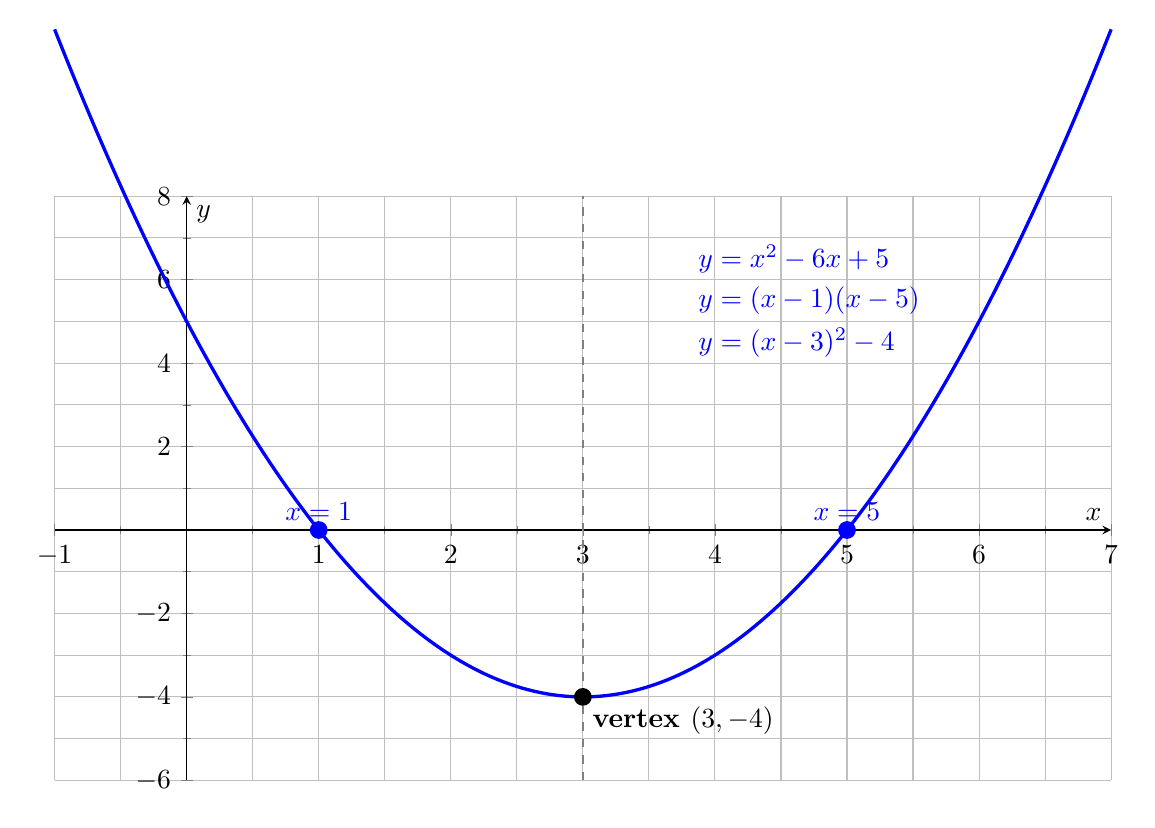
\begin{tikzpicture}
\begin{axis}[
  width=15cm,height=9cm,
  xmin=-1,xmax=7,ymin=-6,ymax=8,
  axis lines=middle,
  xlabel={$x$},ylabel={$y$},
  grid=both,minor tick num=1,
  samples=240,clip=false
]
\addplot[blue,very thick,domain=-1:7]{x^2-6*x+5};
\addplot[gray,dashed,thick] coordinates {(3,-6) (3,8)};
\addplot[blue,only marks,mark=*,mark size=3pt] coordinates {(1,0) (5,0)};
\addplot[black,only marks,mark=*,mark size=3pt] coordinates {(3,-4)};
\node[blue,font=\bfseries,anchor=south] at (axis cs:1,0) {$x=1$};
\node[blue,font=\bfseries,anchor=south] at (axis cs:5,0) {$x=5$};
\node[black,font=\bfseries,anchor=north west] at (axis cs:3,-4) {vertex $(3,-4)$};
\node[blue,font=\bfseries,anchor=west] at (axis cs:3.8,6.5) {$y=x^2-6x+5$};
\node[blue,font=\bfseries,anchor=west] at (axis cs:3.8,5.5) {$y=(x-1)(x-5)$};
\node[blue,font=\bfseries,anchor=west] at (axis cs:3.8,4.5) {$y=(x-3)^2-4$};
\end{axis}
\end{tikzpicture}
\end{document}
